%%
% Copyright (c) 2017 - 2024, Pascal Wagler;
% Copyright (c) 2014 - 2024, John MacFarlane
%
% All rights reserved.
%
% Redistribution and use in source and binary forms, with or without
% modification, are permitted provided that the following conditions
% are met:
%
% - Redistributions of source code must retain the above copyright
% notice, this list of conditions and the following disclaimer.
%
% - Redistributions in binary form must reproduce the above copyright
% notice, this list of conditions and the following disclaimer in the
% documentation and/or other materials provided with the distribution.
%
% - Neither the name of John MacFarlane nor the names of other
% contributors may be used to endorse or promote products derived
% from this software without specific prior written permission.
%
% THIS SOFTWARE IS PROVIDED BY THE COPYRIGHT HOLDERS AND CONTRIBUTORS
% "AS IS" AND ANY EXPRESS OR IMPLIED WARRANTIES, INCLUDING, BUT NOT
% LIMITED TO, THE IMPLIED WARRANTIES OF MERCHANTABILITY AND FITNESS
% FOR A PARTICULAR PURPOSE ARE DISCLAIMED. IN NO EVENT SHALL THE
% COPYRIGHT OWNER OR CONTRIBUTORS BE LIABLE FOR ANY DIRECT, INDIRECT,
% INCIDENTAL, SPECIAL, EXEMPLARY, OR CONSEQUENTIAL DAMAGES (INCLUDING,
% BUT NOT LIMITED TO, PROCUREMENT OF SUBSTITUTE GOODS OR SERVICES;
% LOSS OF USE, DATA, OR PROFITS; OR BUSINESS INTERRUPTION) HOWEVER
% CAUSED AND ON ANY THEORY OF LIABILITY, WHETHER IN CONTRACT, STRICT
% LIABILITY, OR TORT (INCLUDING NEGLIGENCE OR OTHERWISE) ARISING IN
% ANY WAY OUT OF THE USE OF THIS SOFTWARE, EVEN IF ADVISED OF THE
% POSSIBILITY OF SUCH DAMAGE.
%%

%%
% This is the Eisvogel pandoc LaTeX template.
%
% For usage information and examples visit the official GitHub page:
% https://github.com/Wandmalfarbe/pandoc-latex-template
%%

% Options for packages loaded elsewhere
\PassOptionsToPackage{unicode}{hyperref}
\PassOptionsToPackage{hyphens}{url}
\PassOptionsToPackage{dvipsnames,svgnames,x11names,table}{xcolor}
%
\documentclass[
  paper=a4,
  ,captions=tableheading
]{scrartcl}
\usepackage{amsmath,amssymb}
% Use setspace anyway because we change the default line spacing.
% The spacing is changed early to affect the titlepage and the TOC.
\usepackage{setspace}
\setstretch{1.2}
\usepackage{iftex}
\ifPDFTeX
  \usepackage[T1]{fontenc}
  \usepackage[utf8]{inputenc}
  \usepackage{textcomp} % provide euro and other symbols
\else % if luatex or xetex
  \usepackage{unicode-math} % this also loads fontspec
  \defaultfontfeatures{Scale=MatchLowercase}
  \defaultfontfeatures[\rmfamily]{Ligatures=TeX,Scale=1}
\fi
\usepackage{lmodern}
\ifPDFTeX\else
  % xetex/luatex font selection
\fi
% Use upquote if available, for straight quotes in verbatim environments
\IfFileExists{upquote.sty}{\usepackage{upquote}}{}
\IfFileExists{microtype.sty}{% use microtype if available
  \usepackage[]{microtype}
  \UseMicrotypeSet[protrusion]{basicmath} % disable protrusion for tt fonts
}{}
\makeatletter
\@ifundefined{KOMAClassName}{% if non-KOMA class
  \IfFileExists{parskip.sty}{%
    \usepackage{parskip}
  }{% else
    \setlength{\parindent}{0pt}
    \setlength{\parskip}{6pt plus 2pt minus 1pt}}
}{% if KOMA class
  \KOMAoptions{parskip=half}}
\makeatother
\usepackage{xcolor}
\definecolor{default-linkcolor}{HTML}{A50000}
\definecolor{default-filecolor}{HTML}{A50000}
\definecolor{default-citecolor}{HTML}{4077C0}
\definecolor{default-urlcolor}{HTML}{4077C0}
\usepackage[margin=2.5cm,includehead=true,includefoot=true,centering,]{geometry}
\usepackage{color}
\usepackage{fancyvrb}
\newcommand{\VerbBar}{|}
\newcommand{\VERB}{\Verb[commandchars=\\\{\}]}
\DefineVerbatimEnvironment{Highlighting}{Verbatim}{commandchars=\\\{\}}
% Add ',fontsize=\small' for more characters per line
\newenvironment{Shaded}{}{}
\newcommand{\AlertTok}[1]{\textcolor[rgb]{1.00,0.00,0.00}{\textbf{#1}}}
\newcommand{\AnnotationTok}[1]{\textcolor[rgb]{0.38,0.63,0.69}{\textbf{\textit{#1}}}}
\newcommand{\AttributeTok}[1]{\textcolor[rgb]{0.49,0.56,0.16}{#1}}
\newcommand{\BaseNTok}[1]{\textcolor[rgb]{0.25,0.63,0.44}{#1}}
\newcommand{\BuiltInTok}[1]{\textcolor[rgb]{0.00,0.50,0.00}{#1}}
\newcommand{\CharTok}[1]{\textcolor[rgb]{0.25,0.44,0.63}{#1}}
\newcommand{\CommentTok}[1]{\textcolor[rgb]{0.38,0.63,0.69}{\textit{#1}}}
\newcommand{\CommentVarTok}[1]{\textcolor[rgb]{0.38,0.63,0.69}{\textbf{\textit{#1}}}}
\newcommand{\ConstantTok}[1]{\textcolor[rgb]{0.53,0.00,0.00}{#1}}
\newcommand{\ControlFlowTok}[1]{\textcolor[rgb]{0.00,0.44,0.13}{\textbf{#1}}}
\newcommand{\DataTypeTok}[1]{\textcolor[rgb]{0.56,0.13,0.00}{#1}}
\newcommand{\DecValTok}[1]{\textcolor[rgb]{0.25,0.63,0.44}{#1}}
\newcommand{\DocumentationTok}[1]{\textcolor[rgb]{0.73,0.13,0.13}{\textit{#1}}}
\newcommand{\ErrorTok}[1]{\textcolor[rgb]{1.00,0.00,0.00}{\textbf{#1}}}
\newcommand{\ExtensionTok}[1]{#1}
\newcommand{\FloatTok}[1]{\textcolor[rgb]{0.25,0.63,0.44}{#1}}
\newcommand{\FunctionTok}[1]{\textcolor[rgb]{0.02,0.16,0.49}{#1}}
\newcommand{\ImportTok}[1]{\textcolor[rgb]{0.00,0.50,0.00}{\textbf{#1}}}
\newcommand{\InformationTok}[1]{\textcolor[rgb]{0.38,0.63,0.69}{\textbf{\textit{#1}}}}
\newcommand{\KeywordTok}[1]{\textcolor[rgb]{0.00,0.44,0.13}{\textbf{#1}}}
\newcommand{\NormalTok}[1]{#1}
\newcommand{\OperatorTok}[1]{\textcolor[rgb]{0.40,0.40,0.40}{#1}}
\newcommand{\OtherTok}[1]{\textcolor[rgb]{0.00,0.44,0.13}{#1}}
\newcommand{\PreprocessorTok}[1]{\textcolor[rgb]{0.74,0.48,0.00}{#1}}
\newcommand{\RegionMarkerTok}[1]{#1}
\newcommand{\SpecialCharTok}[1]{\textcolor[rgb]{0.25,0.44,0.63}{#1}}
\newcommand{\SpecialStringTok}[1]{\textcolor[rgb]{0.73,0.40,0.53}{#1}}
\newcommand{\StringTok}[1]{\textcolor[rgb]{0.25,0.44,0.63}{#1}}
\newcommand{\VariableTok}[1]{\textcolor[rgb]{0.10,0.09,0.49}{#1}}
\newcommand{\VerbatimStringTok}[1]{\textcolor[rgb]{0.25,0.44,0.63}{#1}}
\newcommand{\WarningTok}[1]{\textcolor[rgb]{0.38,0.63,0.69}{\textbf{\textit{#1}}}}

% Workaround/bugfix from jannick0.
% See https://github.com/jgm/pandoc/issues/4302#issuecomment-360669013)
% or https://github.com/Wandmalfarbe/pandoc-latex-template/issues/2
%
% Redefine the verbatim environment 'Highlighting' to break long lines (with
% the help of fvextra). Redefinition is necessary because it is unlikely that
% pandoc includes fvextra in the default template.
\usepackage{fvextra}
\DefineVerbatimEnvironment{Highlighting}{Verbatim}{breaklines,fontsize=\small,commandchars=\\\{\}}

% add backlinks to footnote references, cf. https://tex.stackexchange.com/questions/302266/make-footnote-clickable-both-ways
\usepackage{footnotebackref}
\usepackage{graphicx}
\makeatletter
\def\maxwidth{\ifdim\Gin@nat@width>\linewidth\linewidth\else\Gin@nat@width\fi}
\def\maxheight{\ifdim\Gin@nat@height>\textheight\textheight\else\Gin@nat@height\fi}
\makeatother
% Scale images if necessary, so that they will not overflow the page
% margins by default, and it is still possible to overwrite the defaults
% using explicit options in \includegraphics[width, height, ...]{}
\setkeys{Gin}{width=\maxwidth,height=\maxheight,keepaspectratio}
% Set default figure placement to htbp
% Make use of float-package and set default placement for figures to H.
% The option H means 'PUT IT HERE' (as  opposed to the standard h option which means 'You may put it here if you like').
\usepackage{float}
\floatplacement{figure}{H}
\makeatother
\setlength{\emergencystretch}{3em} % prevent overfull lines
\providecommand{\tightlist}{%
  \setlength{\itemsep}{0pt}\setlength{\parskip}{0pt}}
\setcounter{secnumdepth}{-\maxdimen} % remove section numbering
\usepackage{bookmark}
\IfFileExists{xurl.sty}{\usepackage{xurl}}{} % add URL line breaks if available
\urlstyle{same}
\hypersetup{
  hidelinks,
  breaklinks=true,
  pdfcreator={LaTeX via pandoc with the Eisvogel template}}
\author{}
\date{}



%%
%% added
%%


%
% for the background color of the title page
%

%
% break urls
%
\PassOptionsToPackage{hyphens}{url}

%
% When using babel or polyglossia with biblatex, loading csquotes is recommended
% to ensure that quoted texts are typeset according to the rules of your main language.
%
\usepackage{csquotes}

%
% captions
%
\definecolor{caption-color}{HTML}{777777}
\usepackage[font={stretch=1.2}, textfont={color=caption-color}, position=top, skip=4mm, labelfont=bf, singlelinecheck=false, justification=raggedright]{caption}
\setcapindent{0em}

%
% blockquote
%
\definecolor{blockquote-border}{RGB}{221,221,221}
\definecolor{blockquote-text}{RGB}{119,119,119}
\usepackage{mdframed}
\newmdenv[rightline=false,bottomline=false,topline=false,linewidth=3pt,linecolor=blockquote-border,skipabove=\parskip]{customblockquote}
\renewenvironment{quote}{\begin{customblockquote}\list{}{\rightmargin=0em\leftmargin=0em}%
\item\relax\color{blockquote-text}\ignorespaces}{\unskip\unskip\endlist\end{customblockquote}}

%
% Source Sans Pro as the default font family
% Source Code Pro for monospace text
%
% 'default' option sets the default
% font family to Source Sans Pro, not \sfdefault.
%
\ifnum 0\ifxetex 1\fi\ifluatex 1\fi=0 % if pdftex
    \usepackage[default]{sourcesanspro}
  \usepackage{sourcecodepro}
  \else % if not pdftex
    \usepackage[default]{sourcesanspro}
  \usepackage{sourcecodepro}

  % XeLaTeX specific adjustments for straight quotes: https://tex.stackexchange.com/a/354887
  % This issue is already fixed (see https://github.com/silkeh/latex-sourcecodepro/pull/5) but the
  % fix is still unreleased.
  % TODO: Remove this workaround when the new version of sourcecodepro is released on CTAN.
  \ifxetex
    \makeatletter
    \defaultfontfeatures[\ttfamily]
      { Numbers   = \sourcecodepro@figurestyle,
        Scale     = \SourceCodePro@scale,
        Extension = .otf }
    \setmonofont
      [ UprightFont    = *-\sourcecodepro@regstyle,
        ItalicFont     = *-\sourcecodepro@regstyle It,
        BoldFont       = *-\sourcecodepro@boldstyle,
        BoldItalicFont = *-\sourcecodepro@boldstyle It ]
      {SourceCodePro}
    \makeatother
  \fi
  \fi

%
% heading color
%
\definecolor{heading-color}{RGB}{40,40,40}
\addtokomafont{section}{\color{heading-color}}
% When using the classes report, scrreprt, book,
% scrbook or memoir, uncomment the following line.
%\addtokomafont{chapter}{\color{heading-color}}

%
% variables for title, author and date
%
\usepackage{titling}
\title{}
\author{}
\date{}

%
% tables
%

%
% remove paragraph indentation
%
\setlength{\parindent}{0pt}
\setlength{\parskip}{6pt plus 2pt minus 1pt}
\setlength{\emergencystretch}{3em}  % prevent overfull lines

%
%
% Listings
%
%


%
% header and footer
%
\usepackage[headsepline,footsepline]{scrlayer-scrpage}

\newpairofpagestyles{eisvogel-header-footer}{
  \clearpairofpagestyles
  \ihead*{}
  \chead*{}
  \ohead*{}
  \ifoot*{}
  \cfoot*{}
  \ofoot*{\thepage}
  \addtokomafont{pageheadfoot}{\upshape}
}
\pagestyle{eisvogel-header-footer}



%%
%% end added
%%

\begin{document}

%%
%% begin titlepage
%%

%%
%% end titlepage
%%



\subsection{EXERCICE 3 (8 points)}\label{exercice-3-8-points}

\emph{Cet exercice porte sur la programmation orientée objet, sur les
arbres binaires de recherche et la récursivité.}

Chaque année, plusieurs courses de chiens de traîneaux sont organisées
sur les terrains enneigés. L'une d'elle, \emph{La Traversée Blanche},
est une course se déroulant en 9 étapes. L'organisateur de cette course
est chargé de créer un programme Python pour aider à la bonne gestion de
l'événement.

\subsubsection{Partie A : la classe
Chien}\label{partie-a-la-classe-chien}

Afin de caractériser un chien, l'organisateur décide de créer une classe
\texttt{Chien} avec les attributs suivants :

\begin{itemize}
\tightlist
\item
  \texttt{id\_chien}, un nombre entier correspondant au numéro attribué
  au chien lors de son inscription à la course ;
\item
  \texttt{nom}, une chaîne de caractères correspondant au nom du chien ;
\item
  \texttt{role}, une chaîne de caractères correspondant au poste occupé
  par le chien : en fonction de sa place dans l'attelage, un chien a un
  rôle bien défini et peut être
  \texttt{\textquotesingle{}leader\textquotesingle{}},
  \texttt{\textquotesingle{}swing\ dog\textquotesingle{}},
  \texttt{\textquotesingle{}wheel\ dog\textquotesingle{}} ou
  \texttt{\textquotesingle{}team\ dog\textquotesingle{}}.
\item
  \texttt{id\_proprietaire}, un nombre entier correspondant au numéro de
  l'équipe.
\end{itemize}

Le code Python incomplet de la classe \texttt{Chien} est donné
ci-dessous.

\begin{Shaded}
\begin{Highlighting}[]
\DecValTok{1}  \KeywordTok{class}\NormalTok{ Chien:}
\DecValTok{2}     \KeywordTok{def} \FunctionTok{\_\_init\_\_}\NormalTok{(}\VariableTok{self}\NormalTok{, id\_chien, nom, role, id\_prop):}
\DecValTok{3}         \VariableTok{self}\NormalTok{.id\_chien }\OperatorTok{=}\NormalTok{ id\_chien}
\DecValTok{4}         \VariableTok{self}\NormalTok{.nom }\OperatorTok{=}\NormalTok{ nom}
\DecValTok{5}         \VariableTok{self}\NormalTok{.role }\OperatorTok{=}\NormalTok{ role}
\DecValTok{6}         \VariableTok{self}\NormalTok{.id\_proprietaire }\OperatorTok{=}\NormalTok{ id\_prop}
\DecValTok{7}     \KeywordTok{def}\NormalTok{ changer\_role(}\VariableTok{self}\NormalTok{, nouveau\_role):}
\DecValTok{8}        \StringTok{"""Change le rôle du chien avec la valeur passée en paramètre."""}
\DecValTok{9}\NormalTok{        ...}
\end{Highlighting}
\end{Shaded}

Voici un extrait des informations dont on dispose sur les chiens
inscrits à la course.

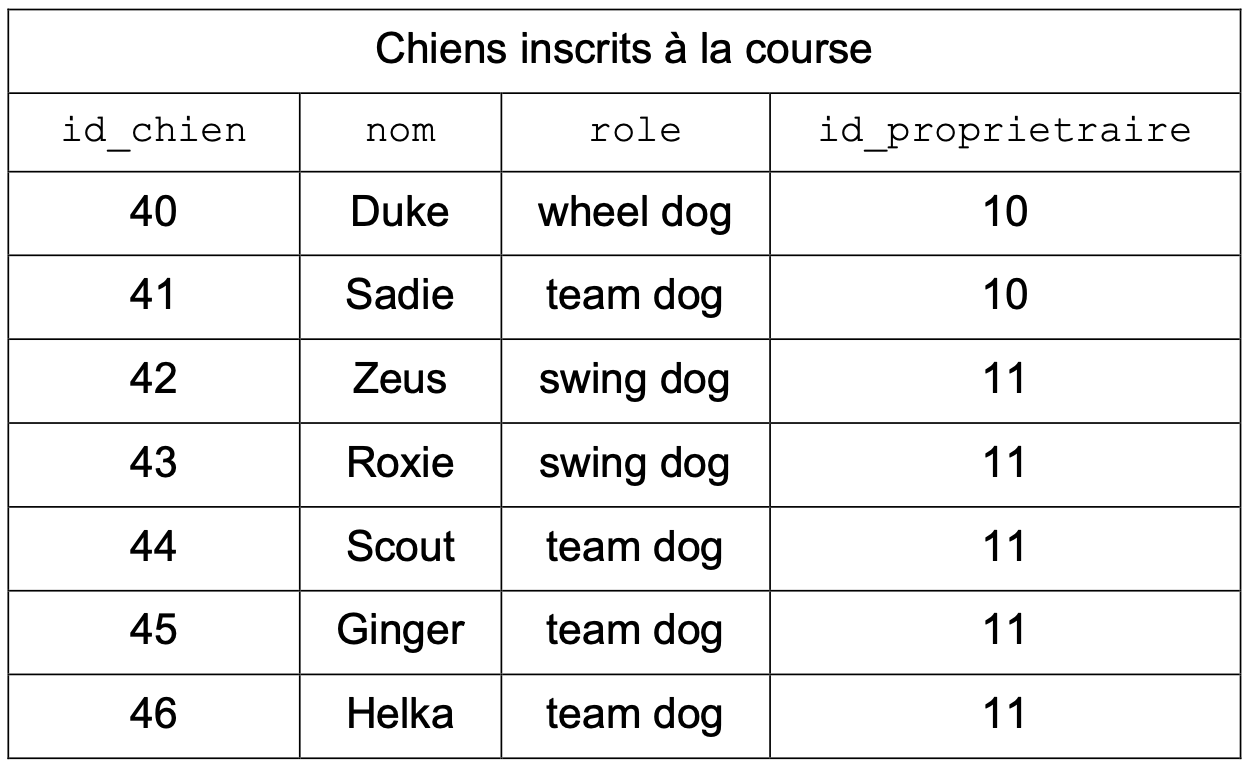
\includegraphics{24-NSIJ1ME1-Ex3-01.png}

Suite aux inscriptions, l'organisateur procède à la création de tous les
objets de type \texttt{Chien} et les stocke dans des variables en
choisissant un nom explicite. Ainsi, l'objet dont l'attribut
\texttt{id\_chien} a pour valeur 40 est stocké dans la variable
\texttt{chien40}.

\begin{enumerate}
\def\labelenumi{\arabic{enumi}.}
\tightlist
\item
  \textbf{Écrire} l'instruction permettant d'instancier l'objet
  \texttt{chien40} caractérisant le chien ayant le numéro d'inscription
  40.
\item
  Selon l'état de fatigue de ses chiens ou du profil de l'étape, le
  \emph{musher} (nom donné à la personne qui conduit le traîneau) peut
  décider de changer le rôle des chiens dans l'attelage.
\end{enumerate}

\textbf{Recopier} et \textbf{compléter} la méthode
\texttt{changer\_role} de la classe \texttt{Chien}.

\begin{enumerate}
\def\labelenumi{\arabic{enumi}.}
\setcounter{enumi}{2}
\tightlist
\item
  Le propriétaire de Duke décide de lui attribuer le rôle de
  \texttt{\textquotesingle{}leader\textquotesingle{}}.
\end{enumerate}

\textbf{Écrire} l'instruction permettant d'effectuer cette modification.

\subsubsection{Partie B : la classe
Equipe}\label{partie-b-la-classe-equipe}

On souhaite à présent créer une classe \texttt{Equipe} ayant les
attributs suivants :

\begin{itemize}
\tightlist
\item
  \texttt{num\_dossard}, un nombre entier correspondant au numéro
  inscrit sur le dossard du musher ;
\item
  \texttt{nom\_equipe}, une chaîne de caractères correspondant au nom de
  l'équipe ;
\item
  \texttt{liste\_chiens}, une liste d'objets de type \texttt{Chien} dont
  chaque élément correspond à un chien au départ de l'étape du jour ;
\item
  \texttt{temps\_etape}, une chaîne de caractères (par exemple
  \texttt{\textquotesingle{}2h34\textquotesingle{}}) représentant le
  temps mis par l'équipe pour parcourir l'étape du jour ;
\item
  \texttt{liste\_temps}, une liste de chaînes de caractères permettant
  de stocker les temps de l'équipe pour chacune des 9 étapes. Cet
  attribut peut, par exemple, contenir la liste :
  \texttt{{[}\textquotesingle{}4h36\textquotesingle{},\ \textquotesingle{}3h57\textquotesingle{},\ \textquotesingle{}3h09\textquotesingle{},\ \textquotesingle{}5h49\textquotesingle{},\ \textquotesingle{}4h45\textquotesingle{},\ \textquotesingle{}3h26\textquotesingle{},\ \textquotesingle{}4h57\textquotesingle{},\ \textquotesingle{}5h52\textquotesingle{},\ \textquotesingle{}4h31\textquotesingle{}{]}}.
\end{itemize}

On donne le code Python suivant de la classe \texttt{Equipe}.

\begin{Shaded}
\begin{Highlighting}[]
\DecValTok{1} \KeywordTok{class}\NormalTok{ Equipe:}
\DecValTok{2}   \KeywordTok{def} \FunctionTok{\_\_init\_\_}\NormalTok{(}\VariableTok{self}\NormalTok{, num\_dossard, nom\_equipe):}
\DecValTok{3}       \VariableTok{self}\NormalTok{.num\_dossard }\OperatorTok{=}\NormalTok{ num\_dossard}
\DecValTok{4}       \VariableTok{self}\NormalTok{.nom\_equipe }\OperatorTok{=}\NormalTok{ nom\_equipe}
\DecValTok{5}       \VariableTok{self}\NormalTok{.liste\_chiens }\OperatorTok{=}\NormalTok{ []}
\DecValTok{6}       \VariableTok{self}\NormalTok{.temps\_etape }\OperatorTok{=} \StringTok{\textquotesingle{}\textquotesingle{}}
\DecValTok{7}       \VariableTok{self}\NormalTok{.liste\_temps }\OperatorTok{=}\NormalTok{ []}
\DecValTok{8}
\DecValTok{9}   \KeywordTok{def}\NormalTok{ ajouter\_chien(}\VariableTok{self}\NormalTok{, chien):}
\DecValTok{10}      \VariableTok{self}\NormalTok{.liste\_chiens.append(chien)}
\DecValTok{11}
\DecValTok{12}  \KeywordTok{def}\NormalTok{ retirer\_chien(}\VariableTok{self}\NormalTok{, numero):}
\DecValTok{13}\NormalTok{      ...}
\DecValTok{14}
\DecValTok{15}  \KeywordTok{def}\NormalTok{ ajouter\_temps\_etape(}\VariableTok{self}\NormalTok{, temps):}
\DecValTok{16}      \VariableTok{self}\NormalTok{.liste\_temps.append(temps)}
\end{Highlighting}
\end{Shaded}

Pour la première étape, le musher de l'équipe numéro 11, représentée en
Python par l'objet \texttt{eq11}, décide de constituer une équipe avec
les quatre chiens identifiés par les numéros 42, 44, 45 et 46. On donne
ci-dessous les instructions Python permettant de créer l'équipe
\texttt{eq11} et l'attelage constitué des 4 chiens précédents.

\begin{Shaded}
\begin{Highlighting}[]
\DecValTok{1}\NormalTok{ eq11 }\OperatorTok{=}\NormalTok{ Equipe(}\DecValTok{11}\NormalTok{, }\StringTok{\textquotesingle{}Malamutes Endurants\textquotesingle{}}\NormalTok{)}
\DecValTok{2}\NormalTok{ eq11.ajouter\_chien(chien42)}
\DecValTok{3}\NormalTok{ eq11.ajouter\_chien(chien44)}
\DecValTok{4}\NormalTok{ eq11.ajouter\_chien(chien45)}
\DecValTok{5}\NormalTok{ eq11.ajouter\_chien(chien46)}
\end{Highlighting}
\end{Shaded}

Malheureusement, le musher s'aperçoit que sa chienne Helka, chien numéro
46, n'est pas au mieux de sa forme et il décide de la retirer de
l'attelage.

\begin{enumerate}
\def\labelenumi{\arabic{enumi}.}
\setcounter{enumi}{3}
\item
  \textbf{Recopier} et \textbf{compléter} la méthode
  \texttt{retirer\_chien} ayant pour paramètre numero, un entier
  correspondant au numéro attribué au chien lors de l'inscription, et
  permettant de mettre à jour l'attribut \texttt{liste\_chiens} après
  retrait du chien dont la valeur de l'attribut \texttt{id\_chien} est
  numero.
\item
  En vous aidant de la fonction précédente, écrire l'instruction qui
  permet de retirer Helka de l'attelage de l'équipe \texttt{eq11}.
\end{enumerate}

On donne à présent le code Python d'une fonction \texttt{convert}
prenant pour paramètre \texttt{chaine}, une chaîne de caractères
représentant une durée, donnée en heure et minute.

On supposera que cette durée est toujours strictement inférieure à 10
heures, temps maximal fixé par le règlement pour terminer une étape.

\begin{Shaded}
\begin{Highlighting}[]
\DecValTok{1} \KeywordTok{def}\NormalTok{ convert(chaine):}
\DecValTok{2}\NormalTok{       heure\_dec }\OperatorTok{=} \BuiltInTok{int}\NormalTok{(chaine[}\DecValTok{0}\NormalTok{]) }\OperatorTok{+} \BuiltInTok{int}\NormalTok{(chaine[}\DecValTok{2}\NormalTok{] }\OperatorTok{+}\NormalTok{ chaine[}\DecValTok{3}\NormalTok{])}\OperatorTok{/}\DecValTok{60}
\DecValTok{3}       \ControlFlowTok{return}\NormalTok{ heure\_dec}
\end{Highlighting}
\end{Shaded}

\begin{enumerate}
\def\labelenumi{\arabic{enumi}.}
\setcounter{enumi}{5}
\tightlist
\item
  \textbf{Indiquer} le résultat renvoyé par l'appel
  \texttt{convert(\textquotesingle{}4h36\textquotesingle{})}.
\item
  \textbf{Écrire} une fonction \texttt{temps\_course} qui prend pour
  paramètre \texttt{equipe} de type \texttt{Equipe} et qui renvoie un
  nombre flottant correspondant au cumul des temps de l'équipe
  \texttt{equipe} à l'issue des 9 étapes de la course.
\end{enumerate}

On rappelle que la classe \texttt{Equipe} dispose d'un attribut
\texttt{liste\_temps}.

\subsubsection{Partie C : classement à l'issue d'une
étape}\label{partie-c-classement-uxe0-lissue-dune-uxe9tape}

Chaque jour, à la fin de l'étape, on décide de construire un Arbre
Binaire de Recherche (ABR) afin d'établir le classement des équipes.
Chaque nœud de cet arbre est un objet de type \texttt{Equipe}.

Dans cet arbre binaire de recherche, en tout nœud :

\begin{itemize}
\tightlist
\item
  toutes les équipes du sous-arbre gauche sont strictement plus rapides
  que ce nœud ;
\item
  toutes les équipes du sous-arbre droit sont moins rapides ou sont à
  égalité avec ce nœud.
\end{itemize}

Voici les temps, en heure et minute, relevés à l'issue de la première
étape :

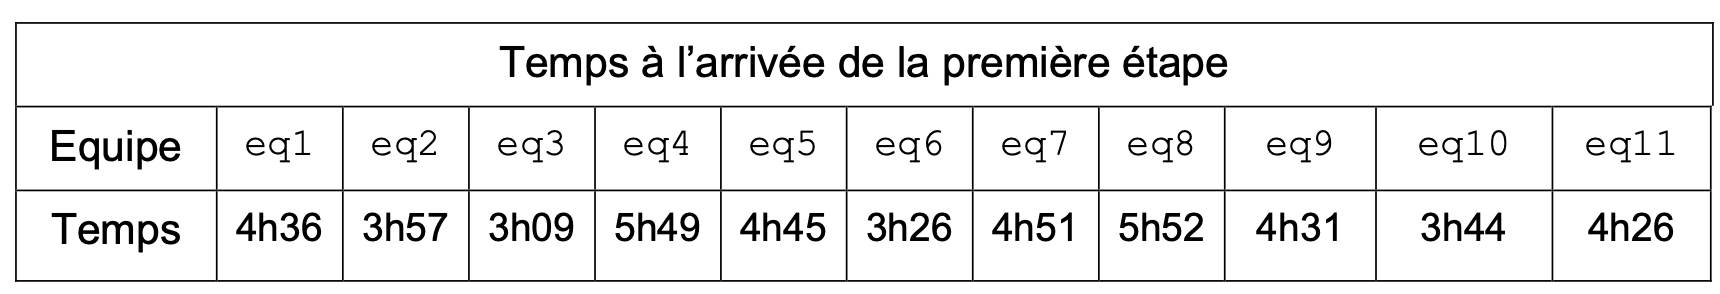
\includegraphics{24-NSIJ1ME1-Ex3-02.png}

Dans l'arbre binaire de recherche initialement vide, on ajoute
successivement, dans cet ordre, les équipes \texttt{eq1}, \texttt{eq2},
\texttt{eq3}, \ldots, \texttt{eq11}, 11 objets de la classe
\texttt{Equipe} tous construits sur le même modèle que l'objet
\texttt{eq11} précédent.

\begin{enumerate}
\def\labelenumi{\arabic{enumi}.}
\setcounter{enumi}{7}
\tightlist
\item
  Dans l'arbre binaire de recherche ci-dessous, les nœuds \texttt{eq1}
  et \texttt{eq2} ont été insérés.
\end{enumerate}

\textbf{Recopier} et \textbf{compléter} cet arbre en insérant les 9
nœuds manquants.

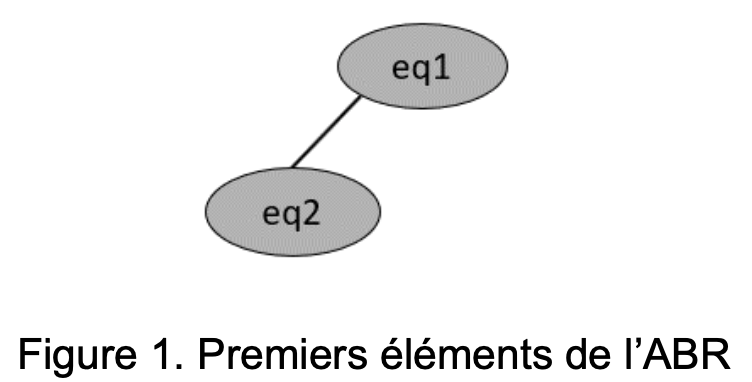
\includegraphics{24-NSIJ1ME1-Ex3-03.png}

\begin{enumerate}
\def\labelenumi{\arabic{enumi}.}
\setcounter{enumi}{8}
\tightlist
\item
  \textbf{Indiquer} quel parcours d'arbre permet d'obtenir la liste des
  équipes classées de la plus rapide à la plus lente.
\end{enumerate}

On donne ci-dessous la classe \texttt{Noeud}, permettant de définir les
arbres binaires :

\begin{Shaded}
\begin{Highlighting}[]
\DecValTok{1} \KeywordTok{class}\NormalTok{ Noeud:}
\DecValTok{2}   \KeywordTok{def} \FunctionTok{\_\_init\_\_}\NormalTok{(}\VariableTok{self}\NormalTok{, equipe, gauche }\OperatorTok{=} \VariableTok{None}\NormalTok{, droit }\OperatorTok{=} \VariableTok{None}\NormalTok{):}
\DecValTok{3}       \VariableTok{self}\NormalTok{.racine }\OperatorTok{=}\NormalTok{ equipe}
\DecValTok{4}       \VariableTok{self}\NormalTok{.gauche }\OperatorTok{=}\NormalTok{ gauche}
\DecValTok{5}       \VariableTok{self}\NormalTok{.droit }\OperatorTok{=}\NormalTok{ droit}
\end{Highlighting}
\end{Shaded}

On donne ci-dessous le code d'une fonction \texttt{construction\_arbre}
qui, à partir d'une liste d'éléments de type \texttt{Noeud} permet
d'insérer successivement chaque nœud à sa place dans l'ABR.

\begin{Shaded}
\begin{Highlighting}[]
\DecValTok{1} \KeywordTok{def}\NormalTok{ construction\_arbre(liste):}
\DecValTok{2}\NormalTok{   a }\OperatorTok{=}\NormalTok{ Noeud(liste[}\DecValTok{0}\NormalTok{])}
\DecValTok{3}   \ControlFlowTok{for}\NormalTok{ i }\KeywordTok{in} \BuiltInTok{range}\NormalTok{(}\DecValTok{1}\NormalTok{,}\BuiltInTok{len}\NormalTok{(liste)):}
\DecValTok{4}\NormalTok{       inserer(a, liste[i])}
\DecValTok{5}   \ControlFlowTok{return}\NormalTok{ a}
\end{Highlighting}
\end{Shaded}

La fonction \texttt{construction\_arbre} fait appel à la fonction
\texttt{inserer} qui prend pour paramètre \texttt{arb}, de type
\texttt{Noeud}, et \texttt{eq}, de type \texttt{Equipe}. Cette fonction
construit le nœud à partir de \texttt{eq} et l'insère à sa place dans
l'ABR.

\begin{Shaded}
\begin{Highlighting}[]
\DecValTok{1} \KeywordTok{def}\NormalTok{ inserer(arb, eq):}
\DecValTok{2}   \StringTok{""" Insertion d\textquotesingle{}une équipe à sa place dans un ABR contenant}
\StringTok{3   au moins un noeud."""}
\DecValTok{4}   \ControlFlowTok{if}\NormalTok{ convert(eq.temps\_etape) }\OperatorTok{\textless{}}\NormalTok{ convert(arb.racine.temps\_etape):}
\DecValTok{5}       \ControlFlowTok{if}\NormalTok{ arb.gauche }\KeywordTok{is} \VariableTok{None}\NormalTok{:}
\DecValTok{6}\NormalTok{           arb.gauche }\OperatorTok{=}\NormalTok{ ...}
\DecValTok{7}       \ControlFlowTok{else}\NormalTok{:}
\DecValTok{8}\NormalTok{           inserer(..., eq)}
\DecValTok{9}   \ControlFlowTok{else}\NormalTok{:}
\DecValTok{10}      \ControlFlowTok{if}\NormalTok{ arb.droit }\KeywordTok{is} \VariableTok{None}\NormalTok{:}
\DecValTok{11}\NormalTok{          arb.droit }\OperatorTok{=}\NormalTok{ Noeud(eq)}
\DecValTok{12}      \ControlFlowTok{else}\NormalTok{:}
\DecValTok{13}\NormalTok{          ...}
\end{Highlighting}
\end{Shaded}

\begin{enumerate}
\def\labelenumi{\arabic{enumi}.}
\setcounter{enumi}{9}
\item
  \textbf{Expliquer} en quoi la fonction \texttt{inserer} est une
  fonction récursive.
\item
  \textbf{Recopier} et \textbf{compléter} les lignes 6, 8 et 13 de la
  fonction \texttt{inserer}.
\item
  \textbf{Recopier} et \textbf{compléter} les lignes 3 et 5 de la
  fonction \texttt{est\_gagnante} ci-dessous qui prend en paramètre un
  ABR \texttt{arbre}, de type \texttt{Noeud}, et qui renvoie le nom de
  l'équipe ayant gagné l'étape.
\end{enumerate}

\begin{Shaded}
\begin{Highlighting}[]
\DecValTok{1} \KeywordTok{def}\NormalTok{ est\_gagnante(arbre):}
\DecValTok{2}     \ControlFlowTok{if}\NormalTok{ arbre.gauche }\OperatorTok{==} \VariableTok{None}\NormalTok{:}
\DecValTok{3}       \ControlFlowTok{return}\NormalTok{ ...}
\DecValTok{4}     \ControlFlowTok{else}\NormalTok{:}
\DecValTok{5}       \ControlFlowTok{return}\NormalTok{ ...}
\end{Highlighting}
\end{Shaded}

\subsubsection{Partie D : classement
général}\label{partie-d-classement-guxe9nuxe9ral}

On décide d'établir un classement général obtenu à partir du cumul des
temps mis par chaque équipe pour parcourir l'ensemble des 9 étapes.

Sur le même principe que l'arbre de la partie précédente, on construit
l'ABR ci-dessous qui permet, grâce au parcours d'arbre approprié,
d'établir ce classement général des équipes.

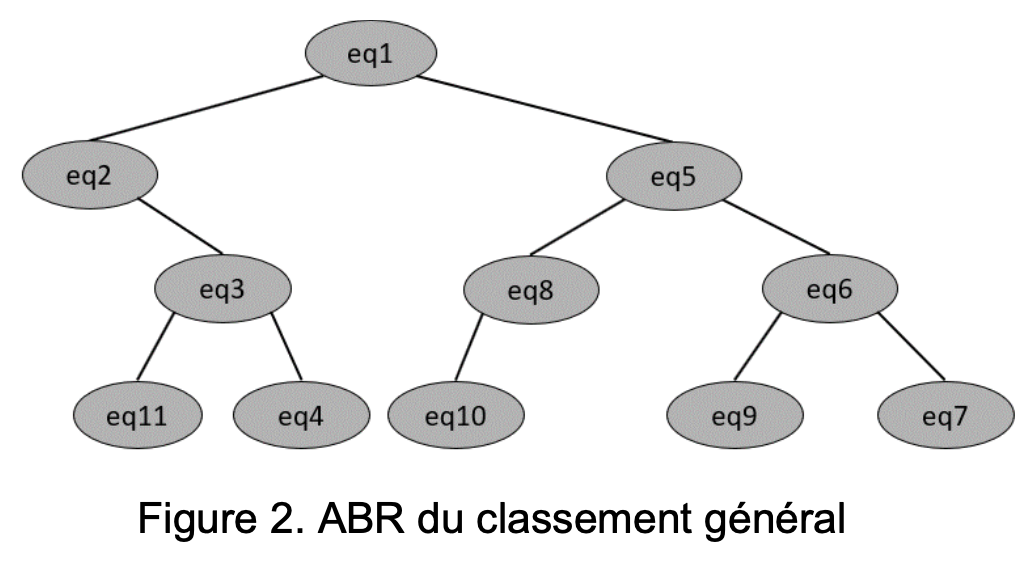
\includegraphics{24-NSIJ1ME1-Ex3-04.png}

Le règlement prévoit la disqualification d'une équipe en cas de
non-respect de celui-ci. Il s'avère que l'équipe 2 et l'équipe 5 doivent
être disqualifiées pour manquement au règlement. Les nœuds \texttt{eq2}
et \texttt{eq5} doivent donc être supprimés de l'ABR précédent.

Pour supprimer un nœud \texttt{N} dans un ABR, trois possibilités se
présentent :

\begin{itemize}
\tightlist
\item
  le nœud \texttt{N} à supprimer est une feuille : il suffit de le
  retirer de l'arbre ;
\item
  le nœud \texttt{N} à supprimer n'a qu'un seul fils : on relie le fils
  de \texttt{N} au père de \texttt{N} et on supprime le nœud \texttt{N}
  ;
\item
  le nœud \texttt{N} à supprimer possède deux fils : on le remplace par
  son successeur (l'équipe qui a le temps immédiatement supérieur) qui
  est toujours le minimum de ses descendants droits.
\end{itemize}

\begin{enumerate}
\def\labelenumi{\arabic{enumi}.}
\setcounter{enumi}{12}
\tightlist
\item
  \textbf{Dessiner} le nouvel arbre de recherche \texttt{a\_final}
  obtenu après suppression des équipes \texttt{eq2} et \texttt{eq5} dans
  l'ABR correspondant au classement général.
\end{enumerate}

L'organisateur souhaite disposer d'une fonction rechercher permettant de
savoir si une équipe a été disqualifiée ou non. On donne les
spécifications de la fonction \texttt{rechercher}, prenant en paramètre
\texttt{arbre} et \texttt{equipe}.

\begin{Shaded}
\begin{Highlighting}[]
\DecValTok{1} \KeywordTok{def}\NormalTok{ rechercher(arbre, equipe):}
\DecValTok{2}   \StringTok{"""}
\StringTok{3       Paramètres}
\StringTok{4       {-}{-}{-}{-}{-}{-}{-}{-}{-}}
\StringTok{5           arbre : un ABR, non vide, de type Noeud, représentant le}
\StringTok{6           classement général.}
\StringTok{7           equipe : un élément, de type Equipe, dont on veut déterminer}
\StringTok{8           l\textquotesingle{}appartenance ou non à l\textquotesingle{}ABR arbre.}
\StringTok{9       Résultat}
\StringTok{10      {-}{-}{-}{-}{-}{-}{-}{-}{-}}
\StringTok{11          Cette fonction renvoie True si equipe est un nœud de arbre,}
\StringTok{12          False sinon.}
\StringTok{13 """}
\DecValTok{14}\NormalTok{ ...}
\end{Highlighting}
\end{Shaded}

Pour cette fonction (\texttt{a\_final} désigne l'arbre obtenu à la
question 13, après suppression des équipes 2 et 5) :

\begin{itemize}
\tightlist
\item
  l'appel \texttt{rechercher(a\_final,\ eq1)} renvoie \texttt{True} ;
\item
  l'appel \texttt{rechercher(a\_final,\ eq2)} renvoie \texttt{False}.
\end{itemize}

\begin{enumerate}
\def\labelenumi{\arabic{enumi}.}
\setcounter{enumi}{13}
\tightlist
\item
  \textbf{Écrire} le code de la fonction
\end{enumerate}

\end{document}